\documentclass[journal,12pt,twocolumn]{IEEEtran}
%
\usepackage{setspace}
\usepackage{gensymb}
%\doublespacing
\singlespacing

%\usepackage{graphicx}
%\usepackage{amssymb}
%\usepackage{relsize}
\usepackage[cmex10]{amsmath}
%\usepackage{amsthm}
%\interdisplaylinepenalty=2500
%\savesymbol{iint}
%\usepackage{txfonts}
%\restoresymbol{TXF}{iint}
%\usepackage{wasysym}
\usepackage{amsthm}
\usepackage{mathrsfs}
\usepackage{txfonts}
\usepackage{stfloats}
\usepackage{steinmetz}
\usepackage{bm}
\usepackage{cite}
\usepackage{cases}
\usepackage{subfig}
%\usepackage{xtab}
\usepackage{longtable}
\usepackage{multirow}
%\usepackage{algorithm}
%\usepackage{algpseudocode}
\usepackage{enumitem}
\usepackage{mathtools}
\usepackage{tikz}
\usepackage{circuitikz}
\usepackage{verbatim}
\usepackage{tfrupee}
\usepackage[breaklinks=true]{hyperref}
%\usepackage{stmaryrd}
\usepackage{tkz-euclide} % loads  TikZ and tkz-base
%\usetkzobj{all}
\usepackage{listings}
    \usepackage{color}                                            %%
    \usepackage{array}                                            %%
    \usepackage{longtable}                                        %%
    \usepackage{calc}                                             %%
    \usepackage{multirow}                                         %%
    \usepackage{hhline}                                           %%
    \usepackage{ifthen}                                           %%
  %optionally (for landscape tables embedded in another document): %%
    \usepackage{lscape}     
\usepackage{multicol}
\usepackage{chngcntr}
%\usepackage{enumerate}

%\usepackage{wasysym}
%\newcounter{MYtempeqncnt}
\DeclareMathOperator*{\Res}{Res}
%\renewcommand{\baselinestretch}{2}
\renewcommand\thesection{\arabic{section}}
\renewcommand\thesubsection{\thesection.\arabic{subsection}}
\renewcommand\thesubsubsection{\thesubsection.\arabic{subsubsection}}

\renewcommand\thesectiondis{\arabic{section}}
\renewcommand\thesubsectiondis{\thesectiondis.\arabic{subsection}}
\renewcommand\thesubsubsectiondis{\thesubsectiondis.\arabic{subsubsection}}

% correct bad hyphenation here
\hyphenation{op-tical net-works semi-conduc-tor}
\def\inputGnumericTable{}                                 %%

\lstset{
%language=C,
frame=single, 
breaklines=true,
columns=fullflexible
}
%\lstset{
%language=tex,
%frame=single, 
%breaklines=true
%}

\begin{document}
%


\newtheorem{theorem}{Theorem}[section]
\newtheorem{problem}{Problem}
\newtheorem{proposition}{Proposition}[section]
\newtheorem{lemma}{Lemma}[section]
\newtheorem{corollary}[theorem]{Corollary}
\newtheorem{example}{Example}[section]
\newtheorem{definition}[problem]{Definition}
%\newtheorem{thm}{Theorem}[section] 
%\newtheorem{defn}[thm]{Definition}
%\newtheorem{algorithm}{Algorithm}[section]
%\newtheorem{cor}{Corollary}
\newcommand{\BEQA}{\begin{eqnarray}}
\newcommand{\EEQA}{\end{eqnarray}}
\newcommand{\define}{\stackrel{\triangle}{=}}
\bibliographystyle{IEEEtran}
%\bibliographystyle{ieeetr}
\providecommand{\mbf}{\mathbf}
\providecommand{\pr}[1]{\ensuremath{\Pr\left(#1\right)}}
\providecommand{\qfunc}[1]{\ensuremath{Q\left(#1\right)}}
\providecommand{\sbrak}[1]{\ensuremath{{}\left[#1\right]}}
\providecommand{\lsbrak}[1]{\ensuremath{{}\left[#1\right.}}
\providecommand{\rsbrak}[1]{\ensuremath{{}\left.#1\right]}}
\providecommand{\brak}[1]{\ensuremath{\left(#1\right)}}
\providecommand{\lbrak}[1]{\ensuremath{\left(#1\right.}}
\providecommand{\rbrak}[1]{\ensuremath{\left.#1\right)}}
\providecommand{\cbrak}[1]{\ensuremath{\left\{#1\right\}}}
\providecommand{\lcbrak}[1]{\ensuremath{\left\{#1\right.}}
\providecommand{\rcbrak}[1]{\ensuremath{\left.#1\right\}}}
\theoremstyle{remark}
\newtheorem{rem}{Remark}
\newcommand{\sgn}{\mathop{\mathrm{sgn}}}
\providecommand{\abs}[1]{\left\vert#1\right\vert}
\providecommand{\res}[1]{\Res\displaylimits_{#1}} 
\providecommand{\norm}[1]{\left\lVert#1\right\rVert}
%\providecommand{\norm}[1]{\lVert#1\rVert}
\providecommand{\mtx}[1]{\mathbf{#1}}
\providecommand{\mean}[1]{E\left[ #1 \right]}
\providecommand{\fourier}{\overset{\mathcal{F}}{ \rightleftharpoons}}
%\providecommand{\hilbert}{\overset{\mathcal{H}}{ \rightleftharpoons}}
\providecommand{\system}{\overset{\mathcal{H}}{ \longleftrightarrow}}
	%\newcommand{\solution}[2]{\textbf{Solution:}{#1}}
\newcommand{\solution}{\noindent \textbf{Solution: }}
\newcommand{\cosec}{\,\text{cosec}\,}
\providecommand{\dec}[2]{\ensuremath{\overset{#1}{\underset{#2}{\gtrless}}}}
\newcommand{\myvec}[1]{\ensuremath{\begin{pmatrix}#1\end{pmatrix}}}
\newcommand{\mydet}[1]{\ensuremath{\begin{vmatrix}#1\end{vmatrix}}}
%\numberwithin{equation}{section}
\numberwithin{equation}{subsection}
%\numberwithin{problem}{section}
%\numberwithin{definition}{section}
\makeatletter
\@addtoreset{figure}{problem}
\makeatother
\let\StandardTheFigure\thefigure
\let\vec\mathbf
%\renewcommand{\thefigure}{\theproblem.\arabic{figure}}
\renewcommand{\thefigure}{\theproblem}
%\setlist[enumerate,1]{before=\renewcommand\theequation{\theenumi.\arabic{equation}}
%\counterwithin{equation}{enumi}
%\renewcommand{\theequation}{\arabic{subsection}.\arabic{equation}}
\def\putbox#1#2#3{\makebox[0in][l]{\makebox[#1][l]{}\raisebox{\baselineskip}[0in][0in]{\raisebox{#2}[0in][0in]{#3}}}}
     \def\rightbox#1{\makebox[0in][r]{#1}}
     \def\centbox#1{\makebox[0in]{#1}}
     \def\topbox#1{\raisebox{-\baselineskip}[0in][0in]{#1}}
     \def\midbox#1{\raisebox{-0.5\baselineskip}[0in][0in]{#1}}
\vspace{3cm}
\title{
ASSIGNMENT 1 - EE5600
	}
\author{ RS Girish - EE20RESCH14005$^{*}$% <-this % stops a space
	}	

\maketitle
\newpage
\tableofcontents
\bigskip
\renewcommand{\thefigure}{\theenumi}
\renewcommand{\thetable}{\theenumi}

\begin{abstract}
This paper contains solution to problem no 17 of Lines and Planes section.
Links to Python codes are available below.  
\end{abstract}
Download python codes using 
\begin{lstlisting}
https://github.com/rsgirishkumar/Assignment1/codes/
\end{lstlisting}
\section{Problem}
Find $m$ if 
\begin{align}
\myvec{2 & 3 }\vec{x}&=11\\
\myvec{2 & -4 }\vec{x}&=-24\\
\myvec{m & -1 }\vec{x}&=-3
\end{align}
\section{Solution}
Given, the system of equations in matrix equation format are as below
\begin{align}
\myvec{2 & 3\\2 & -4\\m & -1}
\vec{x}=
\myvec{11\\-24\\-3}
\end{align}
\textbf{Step1}: Assuming the system of equations are consistent, lets reduce the  augmented matrix [A'b], to find the value of m.
\begin{align*}
\myvec{2 & 3 & 11\\2 & -4 & -24\\m & -1 & -3}
\\R2 -> R2-R1\\
\myvec{2 & 3 & 11\\0 & -7 & -35\\m & -1 & -3}
\\R3 -> 2R3+R1\\
\myvec{2 & 3 & 11\\0 & -7 & -35\\2m+2 & 1 & 5}
\\R3 -> R2+7R3\\
\myvec{2 & 3 & 11\\0 & -7 & -35\\14m+14 & 0 & 0}
\end{align*}
Since the system of equations are assumed consistent,
\begin{align}
14m+14 = 0
\end{align}
\\
\begin{align}
\Rightarrow m=-1
\end{align}
So the system of equations can be re-written as\\
\begin{align}
\myvec{2 & 3 }\vec{x}&=11\\
\myvec{2 & -4 }\vec{x}&=-24\\
\myvec{-1 & -1 }\vec{x}&=-3
\end{align}
\textbf{Step2}:Check the consistency of equations by using the rank of augumented matrix,M=[A'b] and N=matrix [A] as below.
\begin{align*}
N=\myvec{2 & 3\\2 & -4\\-1 & -1}\\
M=\myvec{2 & 3 & 11\\2 & -4 & -24\\-1 & -1 & -3}
\end{align*}
Calculating the rank of matrix M:
\begin{align*}
\myvec{2 & 3 & 11\\2 & -4 & -24\\-1 & -1 & -3}
\\R2 -> R2-R1\\
\myvec{2 & 3 & 11\\0 & -7 & -35\\-1 & -1 & -3}
\\R3 -> 2R3+R1\\
\myvec{2 & 3 & 11\\0 & -7 & -35\\0 & 1 & 5}
\\R3 -> R2+7R3\\
\myvec{2 & 3 & 11\\0 & -7 & -35\\0 & 0 & 0}
\end{align*}
\\No of non zero rows = 2.
\\Hence Rank of matrix(M) =2.
\\Calculating the rank of matrix N:
\begin{align*}
\myvec{2 & 3\\2 & -4\\-1 & -1}
\\R2 -> R2-R1\\
\myvec{2 & 3\\0 & -7\\-1 & -1}
\\R3 -> 2R3+R1\\
\myvec{2 & 3\\0 & -7\\0 & 1}
\\R3 -> R2+7R3\\
\myvec{2 & 3\\0 & -7\\0 & 0}
\end{align*}
\\No of non zero rows = 2.
\\Hence Rank of matrix(N) =2.\\
Since rank of matrix N =2 and M =2, the system of equations are consistent.But,rank(N) = 2 is not equal to total no of rows in matrix(N) i.e.m =3.Since rank(N) != m there exist infinite number of solutions. Of which, the intersection point of any two equations is one of the solutions.
As per ratio of determinants,\\
\begin{align*}
\vec{x}=\frac{\begin{vmatrix}11 & 3\\-24 & -4\\\end{vmatrix}}{\begin{vmatrix}2 & 3\\2 & -4\\\end{vmatrix}}=\frac{-44+72}{-8-6}=\frac{28}{-14}=-2\\
\vec{y}=\frac{\begin{vmatrix}2 & 11\\2 & -24\\\end{vmatrix}}{\begin{vmatrix}2 & 3\\2 & -4\\\end{vmatrix}}=\frac{-48-22}{-8-6}=\frac{70}{14}=5
\end{align*}
The solution is\\
\begin{align}
\myvec{x\\y}\vec{=}\myvec{-2\\5}
\end{align}
The 1.0.3 equation can be substituted with intersection point for verification of solution.
\begin{align*}
\myvec{-1 & -1}&*\myvec{-2\\5}=-3
\end{align*}
Since, the intersection point satisfies the equation, it is one of the solution of all the three equations.\\
The same can be verified from the plot of vectors as below.\\
\\
\textbf{Step3}:The vectors of equations are plotted on 2D axes by taking intersecting points on x and y axes respectively.Intersecting point is given in code.\\
\begin{lstlisting}
https://github.com/rsgirishkumar/Assignment1/codes/assignment1_solution.py
\end{lstlisting}
\begin{figure}[htbp]
  \centering 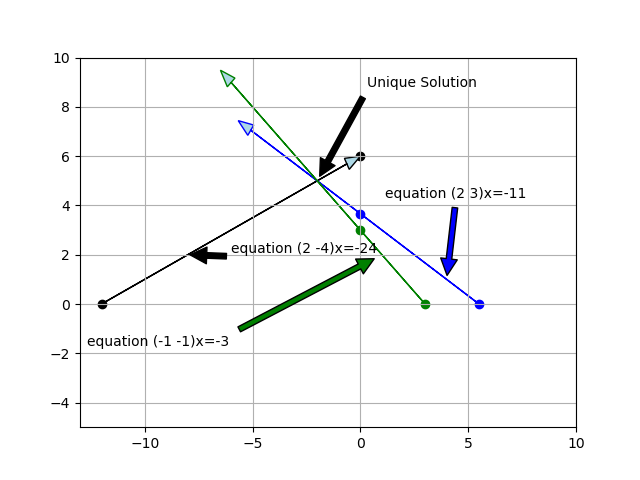
\includegraphics[width=\columnwidth]{assignment1solution_graph1.png}\label{fig0}
  \caption{Three lines intersecting at a point.}\label{cap2}
  \label{fig:Intersection point (-2,5)}
\end{figure} 
\begin{figure}[htbp]
  \centering 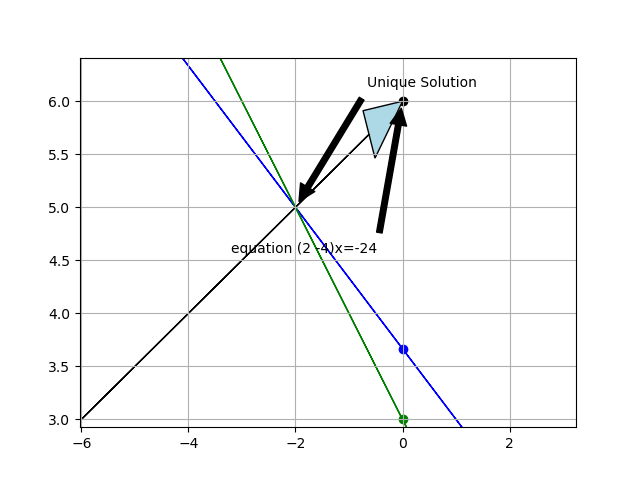
\includegraphics[width=\columnwidth]{assignment1solution_graph.png}\label{fig1}
  \caption{A Clear view.}\label{cap1}
  \label{fig:Intersection point (-2,5)}
\end{figure} 
\end{document}
